\documentclass[]{article}
\usepackage{lmodern}
\usepackage{amssymb,amsmath}
\usepackage{ifxetex,ifluatex}
\usepackage{fixltx2e} % provides \textsubscript
\ifnum 0\ifxetex 1\fi\ifluatex 1\fi=0 % if pdftex
  \usepackage[T1]{fontenc}
  \usepackage[utf8]{inputenc}
\else % if luatex or xelatex
  \ifxetex
    \usepackage{mathspec}
    \usepackage{xltxtra,xunicode}
  \else
    \usepackage{fontspec}
  \fi
  \defaultfontfeatures{Mapping=tex-text,Scale=MatchLowercase}
  \newcommand{\euro}{€}
\fi
% use upquote if available, for straight quotes in verbatim environments
\IfFileExists{upquote.sty}{\usepackage{upquote}}{}
% use microtype if available
\IfFileExists{microtype.sty}{%
\usepackage{microtype}
\UseMicrotypeSet[protrusion]{basicmath} % disable protrusion for tt fonts
}{}
\usepackage[margin=1in]{geometry}
\usepackage{longtable,booktabs}
\usepackage{graphicx}
\makeatletter
\def\maxwidth{\ifdim\Gin@nat@width>\linewidth\linewidth\else\Gin@nat@width\fi}
\def\maxheight{\ifdim\Gin@nat@height>\textheight\textheight\else\Gin@nat@height\fi}
\makeatother
% Scale images if necessary, so that they will not overflow the page
% margins by default, and it is still possible to overwrite the defaults
% using explicit options in \includegraphics[width, height, ...]{}
\setkeys{Gin}{width=\maxwidth,height=\maxheight,keepaspectratio}
\ifxetex
  \usepackage[setpagesize=false, % page size defined by xetex
              unicode=false, % unicode breaks when used with xetex
              xetex]{hyperref}
\else
  \usepackage[unicode=true]{hyperref}
\fi
\hypersetup{breaklinks=true,
            bookmarks=true,
            pdfauthor={Brooks Ambrose},
            pdftitle={Chapter 0 - Aparadigmatic Development of Scholarly Disciplines},
            colorlinks=true,
            citecolor=blue,
            urlcolor=blue,
            linkcolor=magenta,
            pdfborder={0 0 0}}
\urlstyle{same}  % don't use monospace font for urls
\setlength{\parindent}{0pt}
\setlength{\parskip}{6pt plus 2pt minus 1pt}
\setlength{\emergencystretch}{3em}  % prevent overfull lines
\setcounter{secnumdepth}{0}

%%% Use protect on footnotes to avoid problems with footnotes in titles
\let\rmarkdownfootnote\footnote%
\def\footnote{\protect\rmarkdownfootnote}

%%% Change title format to be more compact
\usepackage{titling}

% Create subtitle command for use in maketitle
\newcommand{\subtitle}[1]{
  \posttitle{
    \begin{center}\large#1\end{center}
    }
}

\setlength{\droptitle}{-2em}
  \title{Chapter 0 - Aparadigmatic Development of Scholarly Disciplines}
  \pretitle{\vspace{\droptitle}\centering\huge}
  \posttitle{\par}
  \author{Brooks Ambrose}
  \preauthor{\centering\large\emph}
  \postauthor{\par}
  \predate{\centering\large\emph}
  \postdate{\par}
  \date{October 21, 2015}

\usepackage{booktabs}


\begin{document}

\maketitle


{
\hypersetup{linkcolor=black}
\setcounter{tocdepth}{2}
\tableofcontents
}


\begin{verbatim}
## Loading required package: ngramr
\end{verbatim}

\begin{verbatim}
## Loading required package: ggplot2
\end{verbatim}

\begin{verbatim}
## Loading required package: stargazer
\end{verbatim}

\begin{verbatim}
## 
## Please cite as:
\end{verbatim}

\begin{verbatim}
##  Hlavac, Marek (2015). stargazer: Well-Formatted Regression and Summary Statistics Tables.
\end{verbatim}

\begin{verbatim}
##  R package version 5.2. http://CRAN.R-project.org/package=stargazer
\end{verbatim}

\subsection{Abstract}\label{abstract}

\includegraphics{http://blog.alainntours.fr/IMG/jpg/ch_091107_044_1024px.jpg}

\subsection{Table. Concepts in this
section.}\label{table.-concepts-in-this-section.}

\begin{longtable}[c]{@{}llll@{}}
\toprule
\begin{minipage}[b]{0.14\columnwidth}\raggedright\strut
\textbf{Child}
\strut\end{minipage} &
\begin{minipage}[b]{0.23\columnwidth}\raggedright\strut
\textbf{Social Parent}
\strut\end{minipage} &
\begin{minipage}[b]{0.25\columnwidth}\raggedright\strut
\textbf{Cultural Parent}
\strut\end{minipage} &
\begin{minipage}[b]{0.26\columnwidth}\raggedright\strut
\textbf{Cognitive Parent}
\strut\end{minipage}\tabularnewline
\midrule
\endhead
\begin{minipage}[t]{0.14\columnwidth}\raggedright\strut
Label

Address
\strut\end{minipage} &
\begin{minipage}[t]{0.23\columnwidth}\raggedright\strut
Power

Influence
\strut\end{minipage} &
\begin{minipage}[t]{0.25\columnwidth}\raggedright\strut
Genre

Reference
\strut\end{minipage} &
\begin{minipage}[t]{0.26\columnwidth}\raggedright\strut
Schema

Idea
\strut\end{minipage}\tabularnewline
\bottomrule
\end{longtable}

\section{Paradigms: A High Bar for Scholarly
Disciplines}\label{paradigms-a-high-bar-for-scholarly-disciplines}

Stage-sequential Development of Scholarly Disciplines

\paragraph{Between 1900 and 1925 each American social science discipline
distinguished itself as an autonomous
profession.}\label{between-1900-and-1925-each-american-social-science-discipline-distinguished-itself-as-an-autonomous-profession.}

\paragraph{A key component of the establishment of each as a field was
the development of a pan-disciplinary convention of citing
references.}\label{a-key-component-of-the-establishment-of-each-as-a-field-was-the-development-of-a-pan-disciplinary-convention-of-citing-references.}

We take for granted the use of citations as a currency of information
flow and authorial recognition, but early in the century it was not a
norm to provide precisely codified descriptions of publications.
Citations were often very casual, referencing an author by title and
surname only, and referring to an idea and not any work in particular.
These proto-citations required a contemporary grasp of context to be
intelligible, as do citations today, but they lacked the address-like
codification that would allow the unknowing reader to actually locate
the source in question.

\paragraph{Signpost b/w E\&T}\label{signpost-bw-et}

\paragraph{These battles were hard fought, harder still because each was
a contest on cultural, cognitive, and social
fronts.}\label{these-battles-were-hard-fought-harder-still-because-each-was-a-contest-on-cultural-cognitive-and-social-fronts.}

While all human behavior can be analyzed as consisting in different
ratios of all three components, the institutional development of
professions procedes in a conditional order. While a\footnote{In
  sociology to declare something an institution is to ask how patterns
  of human behavior became regular and to excavate the hidden mechanisms
  that maintain that regularity within limits. Religious practice is
  regulated by the church, political practice by the state (Sewell
  2005:172). Such large scale organizations eclipse the cultures that
  provide the content around which they initially organized. They assure
  their own cultural inputs, and may be open or closed with respect to
  novel culture.} A proto-institution begins to cohere Culture preceeds
cognition in the sense that practices develop tacitly before they are
``recognized'' explicitly, and indeed recognition is, while often
transformative, not actually necessary. On the contrary a cultural
thing, whether an object or a practice, must already exist for it to be
recognized. Likewise cognition, especially classification, preceeds
social control Cultural processes center on human interaction with
meaningfully constituted objects. This far reaching concept is usefully
characterized in the tradition of Geertz where culture exists at the
intersection of symbolically organized thought and concrete practice.
Since Geertz priority has been placed This polarity between real and
ideal may be adapted in a tr

\paragraph{A discipline must cohere culturally before it can
professionalize, and this process occurs in four
stages.}\label{a-discipline-must-cohere-culturally-before-it-can-professionalize-and-this-process-occurs-in-four-stages.}

First, a prototypical set of productions--articles, books and
lectures--had either to be found or invented, and the patterns they
established had to be reproduced without the benefits of consistent
resources or conventions. Second, assembeled productions had to become
recognizable; they had to be labeled and grouped together according to a
consistent symbolism, and that symbolism had to be learned within a
broader milieu. Third, after a symbolic index could be taken for
granted, disciplines would be stillborn if they could not maintain
productivity. Would-be disciples had to produce enough new material to
support an audience intially of peers and then of larger publics.
Fourth, to emerge as professions, disciples had to have a reasonable
chance of being awarded scarce resources within the academy. The ability
to attach the disciplinary label to departments and professorships
marked the beginning of a viable adolescence. If a discipline could
aqcuire the machinery of education it could control the presumption of
its own legitimacy, at least among new generations of students.

\begin{table}[]
\centering
\caption{My caption}
\label{my-label}
\begin{tabular}{lllll}
\hline
                   & \textbf{Aparadigmatic} & \textbf{Transition} & \textbf{Preparadigmatic} & \textbf{Paradigmatic} \\ \hline \hline
\textbf{Cultural}  & Charisma               & Charisma-Genre      & Genre                    & Paradigm              \\
\textbf{Cognitive} & Chaos                  & Chaos-Schema        & Schema                   & Schema                \\
\textbf{Social}    & Autonomy               & Auto-Hetero         & Heteronomy               & Heteronomy            \\ \hline
\end{tabular}
\end{table}

\subsubsection{Table. Stages and their sociocultural
mechanisms.}\label{table.-stages-and-their-sociocultural-mechanisms.}

\begin{longtable}[c]{@{}lll@{}}
\toprule
\begin{minipage}[b]{0.28\columnwidth}\raggedright\strut
\textbf{Stage}
\strut\end{minipage} &
\begin{minipage}[b]{0.23\columnwidth}\raggedright\strut
\textbf{Sensemaking}
\strut\end{minipage} &
\begin{minipage}[b]{0.19\columnwidth}\raggedright\strut
\textbf{Control}
\strut\end{minipage}\tabularnewline
\midrule
\endhead
\begin{minipage}[t]{0.28\columnwidth}\raggedright\strut
\textbf{1. Prototyping}

\textbf{2. Assemblage}

\textbf{3. Facilitation}

\textbf{4. Accumulation}
\strut\end{minipage} &
\begin{minipage}[t]{0.23\columnwidth}\raggedright\strut
Obsession

Recognition

Mastery

Competition
\strut\end{minipage} &
\begin{minipage}[t]{0.19\columnwidth}\raggedright\strut
Private

Peer

Provider

Professional
\strut\end{minipage}\tabularnewline
\bottomrule
\end{longtable}

This study is about the second stage of development, recognition. I
assume that protoypes of disciplinary knowledge were readily available
in the United States by the end of the 19th century, and that the
challenge for disciples was to relabel what had already been
accomplished in an effort to create an occupation out of what was
formally a personal undertaking, an obsession or a pastime.

\section{Cultural Sensemaking}\label{cultural-sensemaking}

\paragraph{In order to regulate their own creative activity, disciples
curated prototypes into sets that drew a boundary, however roughly,
around the tacit definition of what they thought they were
doing.}\label{in-order-to-regulate-their-own-creative-activity-disciples-curated-prototypes-into-sets-that-drew-a-boundary-however-roughly-around-the-tacit-definition-of-what-they-thought-they-were-doing.}

These acts of sorting allowed prototypes to be organized without
requiring the organizer to explain the rules of their order.

\paragraph{Wherever personal sets overlapped the intersection would form
a smaller set of higher
status.}\label{wherever-personal-sets-overlapped-the-intersection-would-form-a-smaller-set-of-higher-status.}

This tendency to overlap one's personal cultural toolkit with that of
others was a form of deference to peers as well as to common culture.
This allowed disciples, without intention, both to claim membership in
the discipline and to indulge in their idiosyncratic variations on the
essence of the discipline. Indeed idiosyncracy would be tolerable only
to the extent that a scholar could in the same breath genuflect to what
was already understood.

\paragraph{While new references to the overlapping set reinforced its
status they also winnowed its
content.}\label{while-new-references-to-the-overlapping-set-reinforced-its-status-they-also-winnowed-its-content.}

Paradoxically by begging to peers that they recognize some novel
prototype scholars would have to also pay homage to the core. They could
not then elevate their own interests above that of the growing stock of
taken for granted knowledge, since introducing something could not
garner attention without attaching it to something old.


\includegraphics{/Users/bambrose/Dropbox/GitHub/manuscripts/Figs/ch0/sensemaking.pdf}

\paragraph{The rejoinder to the claim that nothing can overtake the core
is found in Kuhnian accounts of scientific
revolution.}\label{the-rejoinder-to-the-claim-that-nothing-can-overtake-the-core-is-found-in-kuhnian-accounts-of-scientific-revolution.}

Yet the theory of referential coherence could not be further from that
of paridigmatic coherence. The great advantage of using references as
the currency of disciplinary communication and exchange is that their
meanings can be assumed, and the inevitable disagreements over
interpretation can be easily ignored so long as conversation floats just
above matters of substance. Paridigmatic agreement is not culturally,
that is autonomously, possible unless one makes a very strong empirical
convergence assumption. Exogenous reality must weigh so heavily on the
mind that the concept of interpretation can be dismissed. If however
interpretive variation is the norm then we can also posit that within
limits the same larder satisfies chefs so long as each is free to cook
according to her particular tastes.

\paragraph{Such tastes are not merely metaphorical; an important feature
of this conceptualization is that scholars produce work for their own
consumption first, especially early in the development of a
discipline.}\label{such-tastes-are-not-merely-metaphorical-an-important-feature-of-this-conceptualization-is-that-scholars-produce-work-for-their-own-consumption-first-especially-early-in-the-development-of-a-discipline.}

There must be a point of origin where cultural sensemaking is
idiosyncratic to the creator. It is only with time that multiple
idiosyncracies can be commensurated, and given such commensuration there
can be no expectation that consensus develops to the point of uniformity
in thought even in a solitary thinker not to mention a community of
scholars.

\paragraph{If cultural sensemaking were the only mechanism of
disciplinary coherence then it would draw people together but only
weakly.}\label{if-cultural-sensemaking-were-the-only-mechanism-of-disciplinary-coherence-then-it-would-draw-people-together-but-only-weakly.}

Though the kernel of a core set of references may grow this does not
imply a tendency for disciplines to become closed culturally. What truly
bonds scholars is the opportunity to stand up and be seen through
ceremonies around the core while being otherwise totally invisible when
pursuing idiosyncratic interests.

\subsection{Relevance}\label{relevance}

\section{Cognition}\label{cognition}

\paragraph{Here I attempt to combine internalist and externalist
theories of
culture.}\label{here-i-attempt-to-combine-internalist-and-externalist-theories-of-culture.}

``Art for art's sake'' characterizes the internalist view; cultural
expression is both motivated and regulated by a concept of the object
and standards of quality that, no matter how they got there, are
autonomously held in the mind of the creator. ``Art for the artists's
sake'' characterizes the externalist view, where the interests of the
creator may be multiply determined by a number of social pressures
including fame, fortune, fraud, or force. Many couplets of opposing
forces--knowledge and professions, culture and society, truth and
power--merely replicate this basic distinction.

\paragraph{Yet the internal/external distinction is generic and
restrictive.}\label{yet-the-internalexternal-distinction-is-generic-and-restrictive.}

The underlying references concern how a person might orient herself to
cultural production, and how such productive activity may be embedded in
larger social structures and cultural milieus. I break this distinction
into three simple processes that make creative work easier.

\section{Social Structures}\label{social-structures}

\paragraph{It is during the period where recognition develops that
social control begins to collide with personal
sensemaking.}\label{it-is-during-the-period-where-recognition-develops-that-social-control-begins-to-collide-with-personal-sensemaking.}

This control may at first go no further than a group of peers beginning
to enforce conventions of practice or symbolism by asking or demanding
that a concept be manifest in this way and not that way, or that it not
be expressed at all. If the chief mode of personal sensemaking is
sorting objects into sets of similarity or difference, the nascent form
of social intrusion on cultural sensemaking is attaching labels to the
sets of others. If a sensemaker is exposed to sets with the same label
and different contents then any attending pressure of contradiction
would be most easily resolved by direct interference with someone else's
process of personal sensemaking. Disengaging from the contradiction is
certainly an option, but it is likely that the dopplegangers would find
themselvs at odds again if they inhabit the same milieu.

If there is a weak social force drawing thinkers together at the overlap
of their sensemaking, it will pale in comparison to exogenous sources of
social control that can define cultural relevance by fiat, force, fame,
or facilitation. Even politically motivated ideologies require constant
social control to combat the drift in personal sensemaking.

\paragraph{If a person seeks out social control over their own
sensemaking then they are thoroughly
socialized.}\label{if-a-person-seeks-out-social-control-over-their-own-sensemaking-then-they-are-thoroughly-socialized.}

This tautology may describe some people most of the time and everyone
some of the time. Even if I stipulate that a sensemaker is delighted
when someone else expresses a thought that makes sense to her, such
delight must be predecated on the prior development of recognition, or
else identical thoughts would pass each other unrecognized like ships in
the night.

\paragraph{A cartographic metaphor will be
useful.}\label{a-cartographic-metaphor-will-be-useful.}

The indexing of the set occurs when a set is labeled, and this is
analogous to the name of a contiguous territory on a map. The territory
is defined only by the boundary that encloses it, and no knowledge of
its contents is necessary to refer to the label. Any content discovered
must be categorized de novo, and the boundaries provide the decision
rule to accomplish this. Recognition of bounded content occurs when the
content is given an address. The address need only lead a searcher to a
point of contact with the content, for the address is only a reference
and bears no knowledge of its own.

\paragraph{It is entirely possible that discourse around a set of
references can be sustained without ever referring to underlying
content.}\label{it-is-entirely-possible-that-discourse-around-a-set-of-references-can-be-sustained-without-ever-referring-to-underlying-content.}

The great efficacy of organizing cultural objects into sets of addresses
is that it is much easier to agree on the address than it is to agree on
the character of what is addressed.

\paragraph{In Parsons's terms the addresses are a form of
influence.}\label{in-parsonss-terms-the-addresses-are-a-form-of-influence.}

Influence is a currency bearing social status that allows communication
to occur generically and at a pace faster than would be the case if the
real underlying content had to be mobilized. Money is the archtypical
form of generalized media, allowing exchanges can be defined prior to
the actual mobilization of goods and services.

\paragraph{By organizing cultural history into categories, disciples
solved two important
problems.}\label{by-organizing-cultural-history-into-categories-disciples-solved-two-important-problems.}

First, they sanctioned ignorance; lack of knowledge beyond the curated
set would be no threat to disciplinary credentials. Second, they created
a method of communicating tacit knowledge where formal codification or
training was absent. If a scholar were able to reference the contents of
a curated set in ongoing conversations he would be rewarded with
membership in a self-organized community of scholars including anyone
willing to uphold the legitimacy of the discipline. While variations in
the quantity and quality of set references confer differences in status
iternally, a reference no matter how controversial signaled deference to
the discipline and would be treated as a credential for membership.

\paragraph{Such curation served as a critical factor to scholarly
production in both of its forms, research and
education.}\label{such-curation-served-as-a-critical-factor-to-scholarly-production-in-both-of-its-forms-research-and-education.}

The cultural artifacts of curation left by research were the footnotes
and bibliographies of books and articles, that left by education were
lectures and course syllabi.

\paragraph{Professional activity routinizing the reproduction of the
pattern these protypes
established.}\label{professional-activity-routinizing-the-reproduction-of-the-pattern-these-protypes-established.}

They developed legitimacy for the low level of extant cultural
production, low relative to the subsequent historical growth of
disciplines.

\paragraph{Recognition, a process that amounts to the social
organization of existing cultural
material.}\label{recognition-a-process-that-amounts-to-the-social-organization-of-existing-cultural-material.}

This is the process of genre formation. Though the term is sometimes use
to refer to the entire developing art world or field of cultural
production (Lena and Peterson 2008), \emph{genre} is better reserved to
refer to the development of the cognitive institution alone. Here genres
represent the collision of social constraints with cultural
production.\footnote{In Habermas's terms, genres represent a development
  of system against lifeworld. In Bourdieu's terms, genres are fields,
  specifically the definition of positions to be taken.} The initial
symbols were indexical, allowing productions to be labeled according to
a cogntive categories representing the disciplines. For the U.S. social
sciences, by the end of the ninteenth century symbolism had already been
developed around the . In this regard scholarly disciplines behave
according to a logic of development that has been articulated in the
context of artistic genre.

\paragraph{Tendencies leading to each of these thresholds followed
different yet often intersecting developmental
logics.}\label{tendencies-leading-to-each-of-these-thresholds-followed-different-yet-often-intersecting-developmental-logics.}

\subsection{Typology of Relationships}\label{typology-of-relationships}

\section{Knowledge \& Professions}\label{knowledge-professions}

\subsection{Label: The Disciplinary
Prefixes}\label{label-the-disciplinary-prefixes}

\begin{center}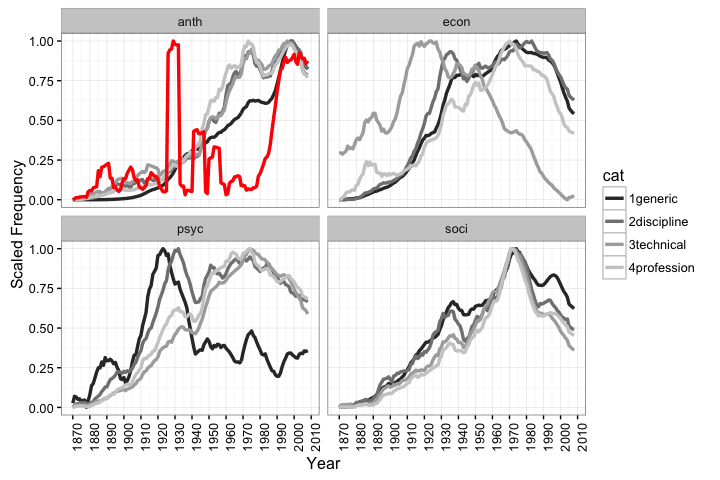
\includegraphics{Figs/ch0/disciplines-1} \end{center}

\subsection{Summary: Cultural and Social
Mechanisms}\label{summary-cultural-and-social-mechanisms}

A cultural action is teleological, autonomously controlled, socially
neutralized, facility constrained, and indeterminant. A social action is
teleological, heteronomously controlled, culturally neutralized,
constrained normatively by prestige, sanctions, and rightness or
competitively by scarcity, acquisition, and attrition, and determinant.
A sociocultural behavior is merely an admixture of the two; on

\subsubsection{Teleology}\label{teleology}

\paragraph{Not all of the things people ``do'' are performances in this
sense.}\label{not-all-of-the-things-people-do-are-performances-in-this-sense.}

Teleological actions have a goal or end known to the subject

\paragraph{Whether knowledge is found or invented is less important than
whether it is addressable; knowledge that is not recoverable might as
well not
exist.}\label{whether-knowledge-is-found-or-invented-is-less-important-than-whether-it-is-addressable-knowledge-that-is-not-recoverable-might-as-well-not-exist.}

Addressing occurs when a source is recoverable via a portable reference
to its location. Because using knowledge tends to reinforce rather than
deplete it, knowledge is only paradoxically scarce. Knowledge is scarce
to the extent that it is easily lost.

\paragraph{Such references went through a process of formalization
wherein casual statements of credit were replaced with precise street
address-like registrations of
locations.}\label{such-references-went-through-a-process-of-formalization-wherein-casual-statements-of-credit-were-replaced-with-precise-street-address-like-registrations-of-locations.}

When for whatever reason citations became precisely codified, especially
in the journal space, it became possible to use references as a form of
currency in the profession. Here the function of citations became
something more than an aide to understanding the text; they became on
one hand raw material for sustained cultural production and on the other
a set of credentials for membership in social science disciplines and
their specialties.

\paragraph{Citations now play several roles, some of which are largely
decoupled from the underlying cultural content to which the citation
ostensibly
points.}\label{citations-now-play-several-roles-some-of-which-are-largely-decoupled-from-the-underlying-cultural-content-to-which-the-citation-ostensibly-points.}

The role of citations at the center of this article concerns how they
are used by researchers to jockey for legitimacy in a competitive
professional field. Citations in this sense are neither forms of
cultural capital, for they may be used without understanding their
significance, nor forms of social capital, because they rarely connote
personal ties among the authors. Instead I consider the claim that
citations are adoptable traits which refer to the abstract social
categories of inclusion and exclusion that form one of the institutional
bases of the academic profession. Insofar as particular lists of
references must be cited to request or signal membership in an extant
professional club, citations become a currency of status exchange.

\paragraph{If a list of citations acts as a credential, there is
variability in the length and content of the list, and this variability
may become the basis of esoteric hierarchies within
disciplines.}\label{if-a-list-of-citations-acts-as-a-credential-there-is-variability-in-the-length-and-content-of-the-list-and-this-variability-may-become-the-basis-of-esoteric-hierarchies-within-disciplines.}

\paragraph{Rewards are stratified into two tiers, the first of which is
socially dominant and the second culturally
dominant.}\label{rewards-are-stratified-into-two-tiers-the-first-of-which-is-socially-dominant-and-the-second-culturally-dominant.}

In the first tier the reward is membership in the professorial
occupation. Given the first, the second reward is prority ranking. This
is the formal recognition that accrues to legendary individuals. A
horizontal stratification attends the segmentation of
disciplines--subdivisions allowing more space for local
heroes.\footnote{Except for rare celebrities that a discipline would
  honor beyond its own boundaries, but again this is a cultural gesture
  whose tangible rewards are irrelevant to the recipient.} (Gustin 1973)

\paragraph{It is only within these subdivisions--including the power
elite as a small and local community of its own--that Bourdieu's fields
of cultural production operate according to a logic of peer
recognition.}\label{it-is-only-within-these-subdivisionsincluding-the-power-elite-as-a-small-and-local-community-of-its-ownthat-bourdieus-fields-of-cultural-production-operate-according-to-a-logic-of-peer-recognition.}

Yet these local communities do not form the larger share of a
professor's quotidian reward. As a sanctioned officer of the academy
professors enjoy influence not with their peers but with their
laity--students and members of the disciplinary public. Horizontal
stratification also allows professors to safely exchange recognition
across disciplinary boundaries without fear of competition.

\section{Empirical Foundations}\label{empirical-foundations}

\paragraph{This brief foray into the different sociocultural functions
of citations may be demonstrated by the observation of the formative
moments of U.S. social
science.}\label{this-brief-foray-into-the-different-sociocultural-functions-of-citations-may-be-demonstrated-by-the-observation-of-the-formative-moments-of-u.s.-social-science.}

The impressions left by the earliest social scientists became a terrain
of disciplines and that could be landscaped but not easily turned over
by future generations. Paradigms or hegemonic cultures developed in the
first half of the 20th century. These paradigms endured even during
times of social upheaval such as the Great Depression and WWII. However,
at the dawn of the 1960s, such monoliths were toppled in quick
succession. For the first time in American history, the cultural
heritage was treated in an a la carte fashion by new generations. What
was really different about the 1960s?

\subsection{A lexical sample}\label{a-lexical-sample}

\paragraph{Each study depends on a database of records of the contents
of
journals.}\label{each-study-depends-on-a-database-of-records-of-the-contents-of-journals.}

This database is compiled from two sources, JSTOR and the Thompson
Reuters Web of Knowledge Social Science Citation Index (WOK).

\paragraph{Ideally, I would analyze the entire stock of recorded
publication material to give the best chance of observing when authors
contravene institutional
boundaries.}\label{ideally-i-would-analyze-the-entire-stock-of-recorded-publication-material-to-give-the-best-chance-of-observing-when-authors-contravene-institutional-boundaries.}

Practically, I must take a sample, however sampled networks are not
small versions of the population network (Handcock and Gile 2010).
Sampling may have the effect of degrading the network cohesion on which
community detection methods depend, such that a method will not detect
the same boundaries in a sample as it would in the population. To avoid
a sampling effect on network cohesion, I draw a full census of articles,
reviews, and book reviews from each journal selected.

\paragraph{Sampling on journals creates another problem, which is to
merely reproduce boundaries coextensive with the journals from which the
articles are
drawn.}\label{sampling-on-journals-creates-another-problem-which-is-to-merely-reproduce-boundaries-coextensive-with-the-journals-from-which-the-articles-are-drawn.}

Even though journals market themselves at catering to particular
disciplines and subfields, I should not assume that authors, editors,
and reviewers always obey these distinctions. If a scholarly field
exists with a grounding in two or more journals, the omission of one may
also degrade its cohesion to the point of rendering its boundaries
undetectable. As an indicator of affiliation among journals, I use
Leydesdorff's (2010)

\paragraph{I should also expect to observe boundaries due to several
other institutional levels higher than journals, like publishers,
disciplines, or national and language
groups.}\label{i-should-also-expect-to-observe-boundaries-due-to-several-other-institutional-levels-higher-than-journals-like-publishers-disciplines-or-national-and-language-groups.}

To provide ample opportunity to observe boundaries existing in the space
between journals and between academic disciplines, I also take a large
sample of journals

\paragraph{To observe some of these high level institutions, I draw sets
of journals from four social science disciplines--anthropology,
sociology, economics, and political science--and I draw these in blocks
from the same
publisher.}\label{to-observe-some-of-these-high-level-institutions-i-draw-sets-of-journals-from-four-social-science-disciplinesanthropology-sociology-economics-and-political-scienceand-i-draw-these-in-blocks-from-the-same-publisher.}

Journals were selected from the disciplinary affiliations signaled in
their titles. From a JSTOR master list of archived materials, journals
were selected if they contained any of the disciplinary prefixes anth-,
soci-, econ-, and poli-. \{\{Though not all journals that are affiliated
with a discipline signal this with a word containing the signature
prefix, those that do are affiliated with a high degree of accuracy.
Soci is an exception, and journals like the Royal Society of Statistics
{[}madeup{]} are excluded.\}\} This list was cross referenced with the
TR WOK database.

\paragraph{To begin it will be useful to consider a theory that is
diametrically opposed to the classification of
groups.}\label{to-begin-it-will-be-useful-to-consider-a-theory-that-is-diametrically-opposed-to-the-classification-of-groups.}

I find one in Bourdieu's essay, \emph{The Social Space and the Genesis
of Groups} \{*Bourdieu:1985wh\}. Bourdieu claims that marxian social
class categories, and their implied boundaries, are analytical
constructs with no real referent in the world. The rules for placing an
uncategorized actor into a class are well established in any number of
class theory traditions. The rules relate to attributes of the actor
which may be independently measured, e.g.~does she sell labor or buy it?
If she sells it, she is a proletarian, if she buys it she is a
bourgeoise. Because these categorical rules are the analyst's, Bourdieu
decries the reification of the boundary between classes so constituted.
Rather than a multidimensional multinomial space, Bourdieu argues that
people actually exist in the world in a multidimensional euclidean
space, where, in capitalism at least, each dimension is a form of
capital. Money, for instance, may be used to place people on a scale and
the difference in their holding defines their distance along one
dimension of that space. cultural capital (the same thing would be true,
mutatis mutandis, of the economic game) determines the aggregate chances
of profit in all the games in which cultural capital is effective,
thereby helping to determine position in social space" (1985:724)
Murkier is Bourdieu's notion of relationship. In the field theory
relationships tend to be competitive bids for profit in a field
constituted by a form of capital. (Shwed and Bearman 2012)

\section{A Realist Epistemology}\label{a-realist-epistemology}

\paragraph{This theory is not empirically
identified.}\label{this-theory-is-not-empirically-identified.}

\paragraph{Cultural products will be
observed}\label{cultural-products-will-be-observed}

\paragraph{Sensemaking will not be
observed}\label{sensemaking-will-not-be-observed}

\paragraph{Social control will not be
observed}\label{social-control-will-not-be-observed}

\paragraph{Sets will be observed}\label{sets-will-be-observed}

\paragraph{Sets are complex outcomes of publication process, involving
inputs from each
mechanism.}\label{sets-are-complex-outcomes-of-publication-process-involving-inputs-from-each-mechanism.}

\paragraph{Mechanism will not be
disentangled}\label{mechanism-will-not-be-disentangled}

\paragraph{Goal is to observe traces of the weakest external boundary.
Field. Art
World.}\label{goal-is-to-observe-traces-of-the-weakest-external-boundary.-field.-art-world.}

\paragraph{Rise and fall of cultural objects as operationalized, not
theorized.}\label{rise-and-fall-of-cultural-objects-as-operationalized-not-theorized.}

\paragraph{Unclear what the operational units mean theoretically, cannot
be known without direct observation of missing
variables.}\label{unclear-what-the-operational-units-mean-theoretically-cannot-be-known-without-direct-observation-of-missing-variables.}

The source data are observations on documents spanning years.

\section*{References}\label{references}
\addcontentsline{toc}{section}{References}

Bourdieu, Pierre. 1985. ``The Social Space and the Genesis of Groups.''
\emph{Theory and Society} 14(6):723--44.

Gustin, Bernard H. 1973. ``Charisma, Recognition, and the Motivation of
Scientists.'' \emph{The American Journal of Sociology} 78(5):1119--34.

Handcock, Mark S. and Krista J. Gile. 2010. ``Modeling social networks
from sampled data.'' \emph{arXiv} stat.AP.

Lena, Jennifer C. and Richard A. Peterson. 2008. ``Classification as
Culture: Types and Trajectories of Music Genres.'' \emph{American
Sociological Review} 73(5):697--718.

Leydesdorff, Loet, Felix de Moya-Anegon, and Vicente P. Guerrero-Bote.
2010. ``Journal Maps on the Basis of Scopus Data: A Comparison with the
Journal Citation Reports of the ISI.'' \emph{Journal Of The American
Society For Information Science And Technology} 61(2):352--69.

Sewell, William H. Jr. 2005. ``The Concept(s) of Culture.'' Pp. 152--74
in \emph{Logics of history}. Chicago: University of Chicago Press.

Shwed, Uri and Peter S. Bearman. 2012. ``Symmetry Is Beautiful.''
\emph{American Sociological Review} 77(6):1064--69.

\end{document}
